\documentclass{assignment}

\course{ECO 120-04}
\name{Lucas Reddinger}
\date{Wednesday 21 November 2022}
\doctitle{Assignment 9: Aggregate supply and demand}

\begin{document}
\RaggedRight

\beginassignment{}

\emph{Due Monday 28 November.} Please submit hardcopy at the beginning of class (11:00 a.m.), or if you prefer, under the door of Wimberly Hall 339C by 10:50 a.m.

\section{Recessions and expansions}

\begin{enumerate}
\item Please define a recessionary period using actual output $Y$ and potential output $Y_p$.
\vfill
\item Please define an expansionary period using actual output $Y$ and potential output $Y_p$.
\vfill
\item Please define the output gap using actual output $Y$ and potential output $Y_p$.
\vfill
\item Please define a recessionary period using the output gap.
\vfill
\item Please define an expansionary period using the output gap.
\vfill
\end{enumerate}

\vspace{-2\baselineskip}
\clearpage

\section{An economy during a recessionary period} \label{sec:recession}

Please graph an economy in a recessionary period using the aggregate supply and demand model.

\begin{enumerate}
\item Begin by drawing and labeling axes.
\item Draw and label an aggregate demand (AD) and short-run aggregate supply (SRAS) curves.
\item Label the aggregate price level $P^*_0$ and the actual output level $Y^*_0$.
\item In a recession, is potential output $Y_p$ above or below actual output $Y^*_0$? \hfill \underline{\hspace{1.5in}}
\item Add a long-run aggregate supply (LRAS) curve to your graph, and label $Y_p$.
\end{enumerate}

\vfill

\begin{center}
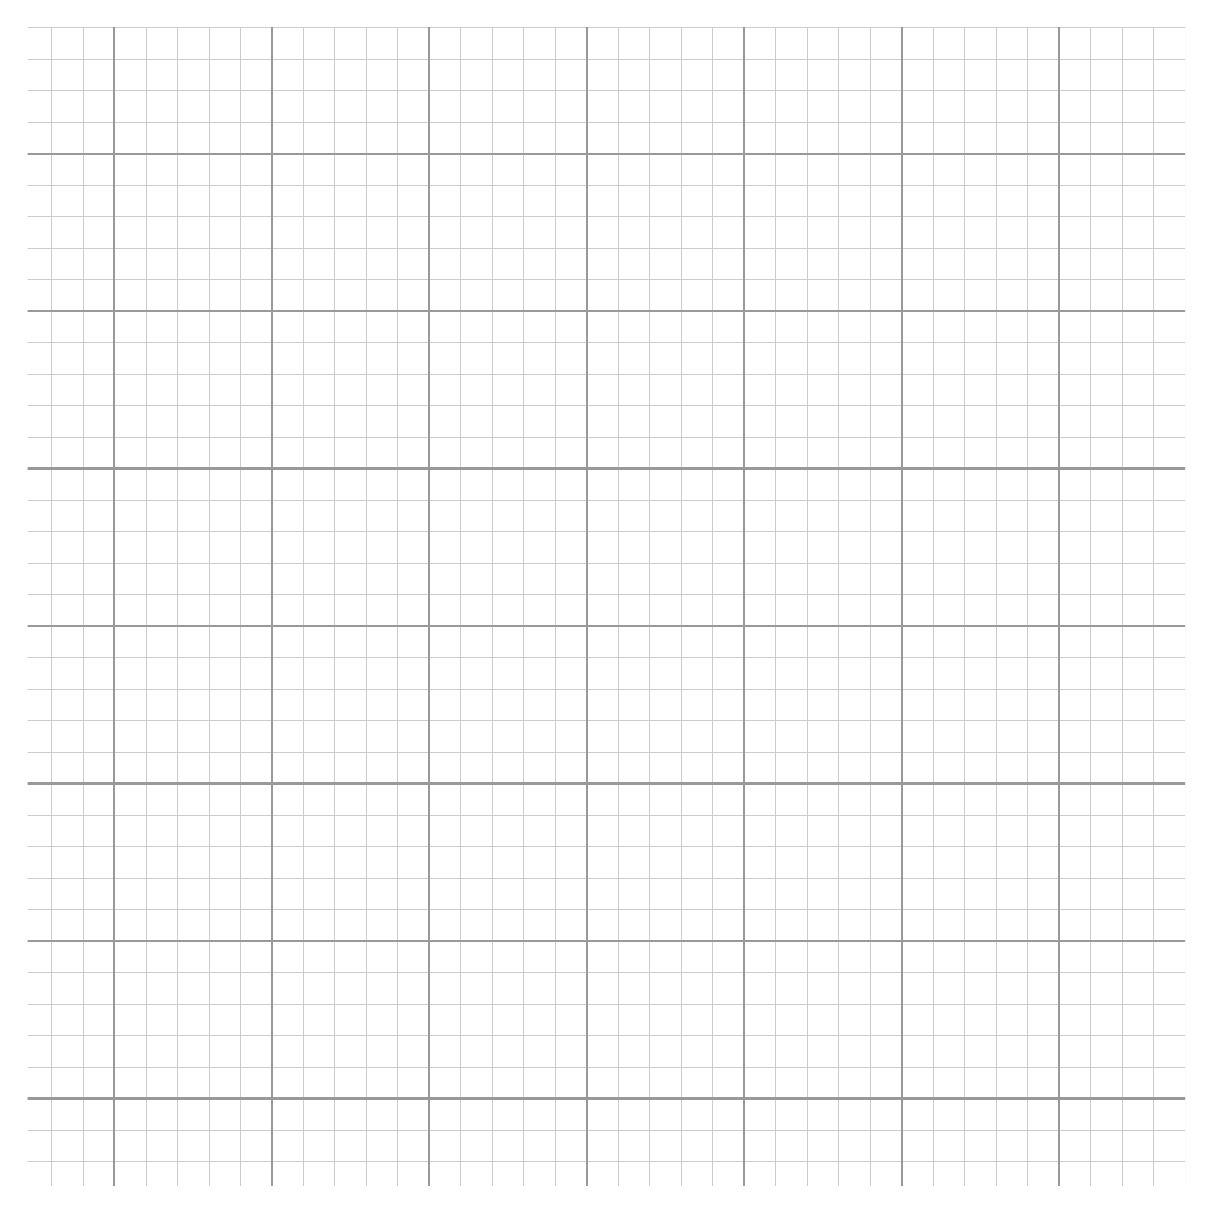
\begin{tikzpicture}[x=3mm, y=3mm]
\clip(3,3) rectangle (52,52);
\draw[step=4mm, very thin, black!20!white] (0,0) grid (60,120);
\draw[step=20mm, thick, black!40!white] (0,0) grid (60,120);
\end{tikzpicture}
\end{center}

\clearpage

\section{An economy during an expansionary period}\label{sec:expansion}

Please graph an economy in an expansionary period using the aggregate supply and demand model.

\begin{enumerate}
\item Begin by drawing and labeling axes.
\item Draw and label an aggregate demand (AD) and short-run aggregate supply (SRAS) curves.
\item Label the aggregate price level $P^*_0$ and the actual output level $Y^*_0$.
\item In an expansion, is potential output $Y_p$ above or below actual output $Y^*_0$? \hfill \underline{\hspace{1.5in}}
\item Add a long-run aggregate supply (LRAS) curve to your graph, and label $Y_p$.
\end{enumerate}

\vfill

\begin{center}
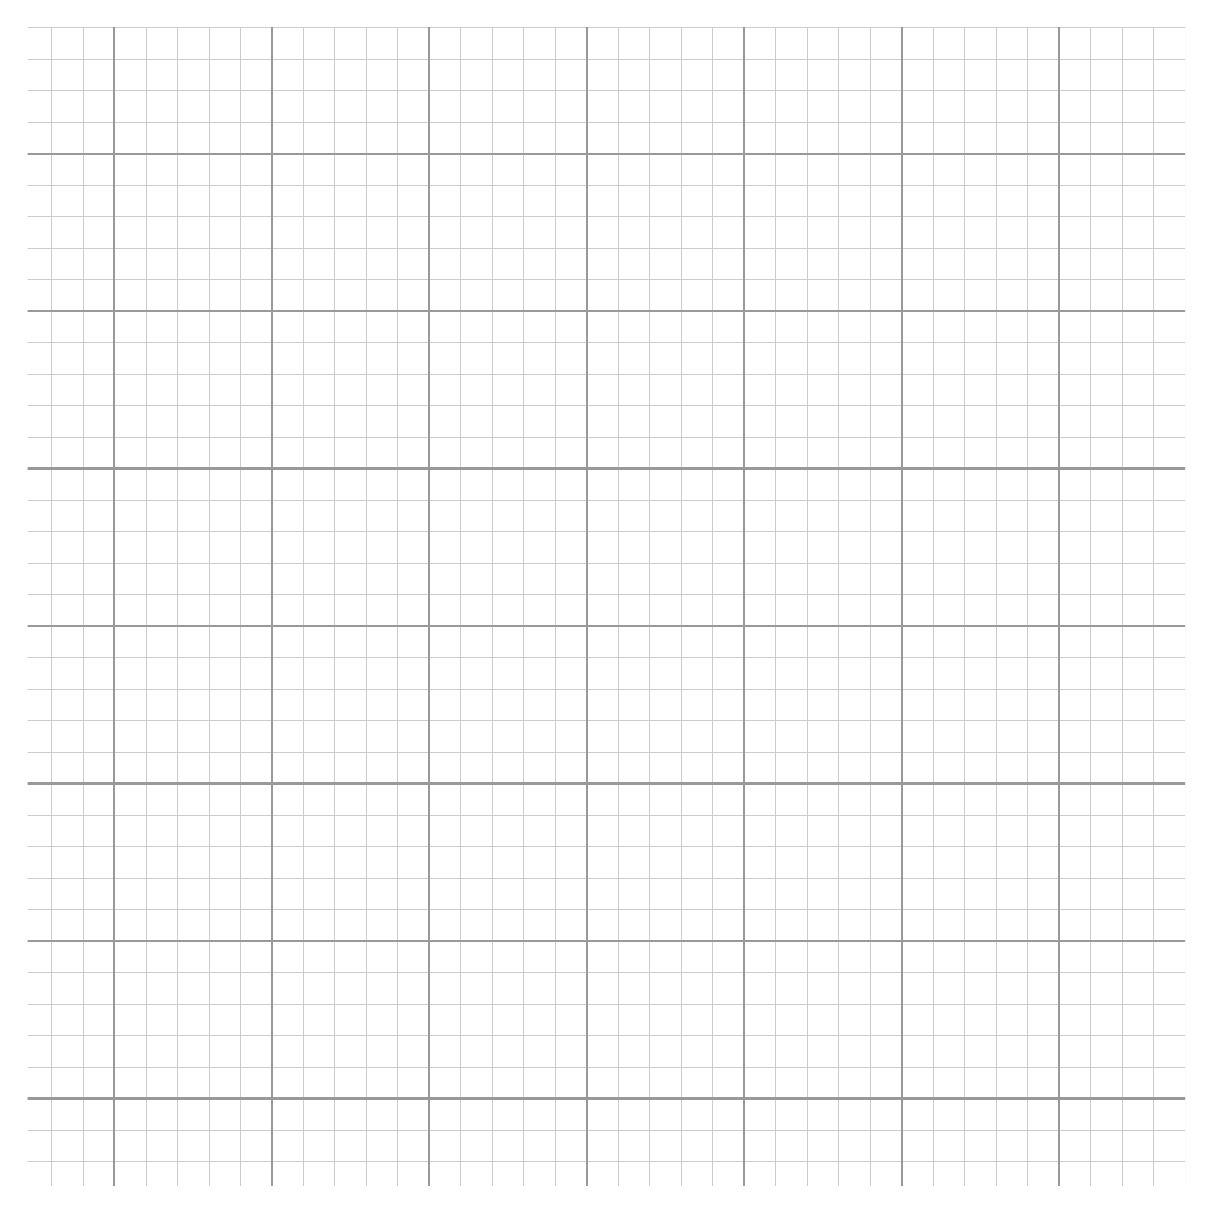
\begin{tikzpicture}[x=3mm, y=3mm]
\clip(3,3) rectangle (52,52);
\draw[step=4mm, very thin, black!20!white] (0,0) grid (60,120);
\draw[step=20mm, thick, black!40!white] (0,0) grid (60,120);
\end{tikzpicture}
\end{center}

\section{The short-run and the long-run}

\begin{enumerate}

\item What characterizes the short-run in the aggregate supply and demand (AS and AD) model?

\vfill

\item Which curve shifts as nominal wages change?

\vfill

\item In which direction does the curve shift \emph{when nominal wages increase}?

\vspace{1.0\baselineskip}
The \underline{\hspace{2in}} curve shifts \underline{\hspace{2in}}.
\vspace{1.0\baselineskip}

\item In which direction does the curve shift \emph{when nominal wages decrease}?

\vspace{1.0\baselineskip}
The \underline{\hspace{2in}} curve shifts \underline{\hspace{2in}}.
\vspace{1.0\baselineskip}

\item In long-run equilibrium, $Y=Y_p$. Revisit \cref{sec:recession}, with \emph{an economy in a recessionary period}. Suppose that wages adjust so that the economy returns to long-run equilibrium. Consider what shift would be necessary to make $Y=Y_p$. Graph this shift, and label the new price level $P^*_1$ and new actual output level $Y^*_1$. Did wages increase or decrease?

\vfill

\item In long-run equilibrium, $Y=Y_p$. Revisit \cref{sec:expansion}, with \emph{an economy in an expansionary period}. Suppose that wages adjust so that the economy returns to long-run equilibrium. Consider what shift would be necessary to make $Y=Y_p$. Graph this shift, and label the new price level $P^*_1$ and new actual output level $Y^*_1$. Did wages increase or decrease?

\vfill

\vspace{-2\baselineskip}
\clearpage

\end{enumerate}

\end{document}
